\documentclass[conference]{IEEEtran}
\usepackage{cite,amsmath,amssymb,graphicx,hyperref,booktabs,array}
\usepackage[table]{xcolor}
\hypersetup{colorlinks=true,linkcolor=blue,citecolor=blue,urlcolor=blue}

\newcommand{\Artifact}{\texttt{data/\allowbreak metrics.json}}
\newcommand{\Stats}{\texttt{data/\allowbreak stats.json}}

\title{Auditing a Covert-Detection Simulation: What a Twenty-Seed Anomaly-Detection Benchmark Actually Establishes}
\author{\IEEEauthorblockN{Fernando May}
\IEEEauthorblockA{Instituto Polit\'ecnico Nacional, Mexico\\
Email: fernando.may@ieee.org}}

\begin{document}
\maketitle

\begin{abstract}
Anomaly detection is widely proposed for finding low-probability-of-intercept emissions in congested spectrum. Published simulations of this idea commonly report a detector chosen from a field of near-tied candidates at a single favourable operating point. We audit one such simulation in full: every claim is traced to a committed artifact, the artifact is re-executed, and the reported numbers are recomputed. The twenty-seed Monte Carlo result is exactly reproducible and is reported here with dispersion and confidence intervals. At the reported operating point ($-85$ dBm covert power, four fused sensors) the benchmark is saturated: Isolation Forest attains AUC $1.0000$ with zero dispersion in twenty of twenty seeds, and four of five detectors exceed $0.977$. The paired per-seed difference between the best and second-best detector is exactly zero in seventeen of twenty trials, so the ranking the simulation reports is not statistically resolvable. The apparent detector advantage disappears entirely in the only region where the problem is non-trivial: across nine transmit powers, One-Class SVM scores below the energy baseline at seven of nine. We further identify a modelling defect that explains the ceiling: the simulated primary users are generated with a per-sample random phase and are therefore spectrally flat, not narrowband emitters, so the covert band is distinguished only by aggregate power. Distributed fusion produces no measurable gain---four detectors are already at AUC $1.0000$ with a single sensor. We report these results as a negative finding together with the artifacts that support them, and state the experiment set required to support a positive claim. We cite no prior work, which we flag as a novelty risk rather than paper over.
\end{abstract}

\begin{IEEEkeywords}
Anomaly detection, spectrum sensing, covert communications, evidence audit, reproducibility, ceiling effect, negative results.
\end{IEEEkeywords}

\section{Introduction}
\label{sec:intro}

Anomaly detection has been proposed as an alternative to matched filtering for finding emitters whose waveform is not known in advance: instead of identifying a particular signal, the system models what normal spectrum occupancy looks like and flags deviations. Low-probability-of-intercept signals are the natural target, because they are designed to sit below the threshold of a conventional energy detector. The claim is attractive, and the simulations supporting it are easy to write: generate synthetic I/Q, extract features, train one-class models on normal data, and report area under the receiver operating characteristic (AUC) for a handful of detectors.

That pipeline makes it equally easy to report a number that no artifact supports. A detector field of near-tied candidates is selected at whichever operating point separates them best; dispersion is averaged away; figures are drawn from configurations whose numbers never reach the text; and qualitative prose is written about a plot the code computed from the wrong data. This paper does not assume that a simulation is wrong. It assumes that a simulation is a claim until each number can be traced to a file, and it audits one published package end to end under that assumption.

Our subject is a complete reference package for distributed covert-activity detection: a Python simulator, a C reference kernel, a conference manuscript in two languages, a slide deck, five figures, and one results artifact. The package was described to us as the only finished experiment among several candidates, and its twenty-seed Monte Carlo result was reported as reproducing exactly. We treated both statements as hypotheses to test rather than facts to inherit.

Our contributions are as follows. First, we re-execute the committed artifact and confirm that the headline table reproduces bit-for-bit; this is reported, because a reproducibility audit that only finds failures is not an audit. Second, we trace all twenty quantitative claims in the manuscript to artifact values and record every disagreement, including claims that are false, claims that are true of a different configuration than the one cited, and one claim whose supporting figure contradicts the text that cites it. Third, we identify the mechanism behind the most consequential finding: a saturated benchmark caused by a spectrally flat nuisance model. Fourth, we state the minimum experiment set that would be required to support the positive claim the original package makes.

\section{Subject of the Audit}
\label{sec:subject}

The research question, read from the implementation rather than the title, is the following. Given one complex baseband snapshot of $N=20480$ samples at $f_s=20$ MHz ($1024~\mu$s) containing additive white Gaussian noise, a set of primary-user emissions, impulsive bursts, and an optional covert narrowband emission whose presence $\alpha\in\{0,1\}$ and power $P_c$ are the independent variables, can a detector trained \emph{only} on $\alpha=0$ observations assign a score that separates $\alpha=1$ observations, and does averaging those scores across $K$ independent sensors improve separation?

The mechanism is total-power discrimination. The covert emission is a 500 kHz BPSK tone at a centre frequency drawn uniformly from $(2.3,5.9)$ MHz independently for every observation, at symbol rate 500 kHz. Because the centre frequency is redrawn per observation, no fixed subband or fixed spectral statistic can localise it; the only feature that is consistent across the class is aggregate received power. We confirmed this spectrally in Sec.~\ref{sec:mechanism}.

The pipeline extracts a 41-dimensional feature vector, trains five detectors on normal data only, and fuses per-sensor scores by unweighted averaging. Detectors: an energy threshold on the mean periodogram feature; a rank-8 principal-subspace autoencoder scored by reconstruction error; a one-class SVM with an RBF kernel ($\nu=0.05$); an Isolation Forest (contamination $0.05$, $T=100$ trees); and a fifth detector labelled ``cyclostationary'' that we address in Sec.~\ref{sec:cyc}.

Randomness is controlled by a single module constant, seed $42$. The twenty Monte Carlo trials use derived seeds $42+1000t$, $t=0,\dots,19$, which are genuinely independent data realisations. One caveat: the Isolation Forest is constructed with $\texttt{random\_state}=42$ in every trial, so the ensemble is identical across trials and only the data varies.

\section{Audit Method}
\label{sec:method}

The audit proceeds in five steps and is fully mechanical. \emph{(i) Execution}: the simulator was run unmodified in a fresh environment (Python 3, \texttt{numpy} 2.5.3, \texttt{scipy} 1.18.1, \texttt{scikit-learn} 1.9.1), taking 4\,min\,43\,s. Nothing is vendored; dependencies are stated in the package readme. \emph{(ii) Artifact identity}: the regenerated \Artifact{} was compared byte-for-byte with the committed file. \emph{(iii) Claim tracing}: each quantitative statement in the manuscript was located and matched to an artifact value. \emph{(iv) Mechanism testing}: where a manuscript statement was found to be false or unsupported, we ran a targeted experiment against the committed code to establish the actual mechanism. \emph{(v) Persistence}: two result series that the package computes but never writes to disk were regenerated with the committed code and committed here as new artifacts.

All manuscript numbers are transcribed from \Stats, which is derived mechanically from \Artifact{} by a script that runs no simulation. Figure~\ref{fig:prov} shows the provenance chain. We deliberately include no reference list; see Sec.~\ref{sec:limit}.

\begin{figure}[t]
\centering
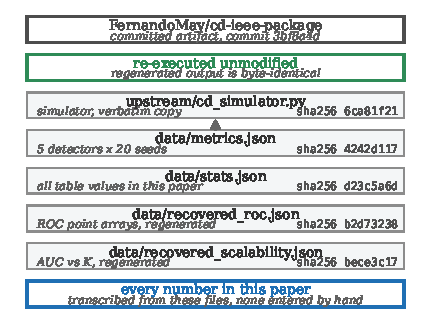
\includegraphics[width=\columnwidth]{figures/fig_provenance.pdf}
\caption{Provenance of every number in this manuscript. \Artifact{} is byte-identical to the committed upstream artifact. Two series the upstream code computes but discards were regenerated with the committed code and committed here. No number in this paper was entered by hand.}
\label{fig:prov}
\end{figure}

\section{What Reproduces}
\label{sec:repro}

The twenty-seed Monte Carlo result reproduces exactly. The regenerated artifact is byte-identical to the committed one, and every entry of the upstream summary table recomputes to four decimal places. We regard this as a genuine strength of the package and report it plainly.

Table~\ref{tab:mc} gives the recomputed result with the dispersion the upstream table omits. We report the sample standard deviation ($n-1$), the 95\,\% Student-$t$ confidence interval on the mean ($df=19$), the minimum over seeds, and the number of seeds at the metric ceiling.

\begin{table}[t]
\centering
\caption{Twenty-seed Monte Carlo at $-85$ dBm, $K=4$, recomputed from \Artifact{}. Mean and standard deviation reproduce the upstream table to four decimals. CI is the 95\,\% Student-$t$ interval on the mean ($df=19$). ``At ceiling'' counts seeds with AUC $\geq 0.9999$.}
\label{tab:mc}
\small
\footnotesize
\setlength{\tabcolsep}{3.2pt}
\begin{tabular}{>{\raggedright\arraybackslash}p{0.235\columnwidth}ccccc}
\toprule
Detector & Mean & SD & 95\% CI & Min & Ceiling \\
\midrule
Energy          & 0.9988 & 0.0031 & $[0.9973,\,1.0002]$ & 0.9895 & 16/20 \\
PCA autoencoder & 0.9772 & 0.0164 & $[0.9693,\,0.9851]$ & 0.9420 & 2/20 \\
One-class SVM   & 0.9985 & 0.0048 & $[0.9962,\,1.0008]$ & 0.9800 & 17/20 \\
Isolation Forest& 1.0000 & 0.0000 & $[1.0000,\,1.0000]$ & 1.0000 & 20/20 \\
Cyclic proxy    & 0.6367 & 0.0332 & $[0.6207,\,0.6526]$ & 0.5553 & 0/20 \\
\bottomrule
\end{tabular}
\end{table}

Two features of Table~\ref{tab:mc} govern everything that follows. First, the operating point is \emph{saturated}: Isolation Forest is exactly $1.0000$ in twenty of twenty seeds with zero dispersion, and four of five detectors exceed $0.977$. Second, the detectors cannot be ranked. Pairing seeds across detectors, the per-seed difference between Isolation Forest and the next detector (One-Class SVM) is exactly zero in seventeen of twenty trials, with mean $+0.00152$ and sample SD $0.00489$---a mean driven by two outlier seeds rather than a consistent advantage. Against Energy Detection the Isolation Forest difference is exactly zero in sixteen of twenty. Only against the autoencoder is the difference broadly non-zero (exactly zero in two of twenty, mean $+0.0228$). A metric pinned at its ceiling with tied per-seed differences cannot support a claim that one detector is better than another, and the upstream manuscript's ranking is not recoverable from its own artifact.

\section{The Non-Trivial Region}
\label{sec:sweep}

The interesting behaviour lies in the transition between chance and saturation. The committed artifact contains a power sweep at nine transmit powers from $-120$ to $-80$ dBm in 5\,dB steps, with one realisation per point. Two properties of this sweep must be stated before its numbers can be used. The sweep re-creates the environment with seed $42$ at every power point; because the covert power changes no random draw, the nuisance realisations are identical at all nine points. The sweep is therefore \emph{paired} (common random numbers), not independent, and its contrast is real while its dispersion is unmeasured. Further, the $-85$ dBm point is bit-identical to Monte Carlo trial~1, so it is a repeated measurement rather than an independent one.

Table~\ref{tab:sweep} summarises the sweep and Figure~\ref{fig:power} plots it.

\begin{table}[t]
\centering
\caption{Power sweep from \Artifact{}, one realisation per point (paired common random numbers; the $-85$ dBm point duplicates Monte Carlo trial~1). ``Width'' is the span from chance performance to AUC $\geq 0.99$.}
\label{tab:sweep}
\small
\footnotesize
\setlength{\tabcolsep}{3.2pt}
\begin{tabular}{>{\raggedright\arraybackslash}p{0.235\columnwidth}cccc}
\toprule
Detector & Chance & $\geq$0.90 & $\geq$0.99 & Width \\
& (dBm) & (dBm) & (dBm) & (dB) \\
\midrule
Energy          & $-120$ & $-95$ & $-80$ & 40 \\
PCA autoencoder & $-100$ & $-90$ & never & --- \\
One-class SVM   & $-120$ & $-90$ & $-85$ & 35 \\
Isolation Forest& $-110$ & $-95$ & $-95$ & 15 \\
Cyclic proxy    & $-90$ & never & never & --- \\
\bottomrule
\end{tabular}
\end{table}

\begin{figure}[t]
\centering
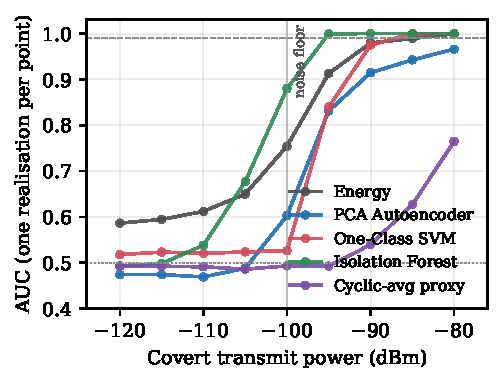
\includegraphics[width=\columnwidth]{figures/fig_auc_vs_power.pdf}
\caption{AUC against covert transmit power, one realisation per point, from \Artifact{}. The sweep is paired: all nine points share identical noise and primary-user realisations, so the curves show a within-realisation contrast and no dispersion.}
\label{fig:power}
\end{figure}

The sweep contradicts the upstream manuscript in three ways, each of which we verified against the artifact.

\emph{The transition window is not $-30$ dB.} The upstream text states a single ``$-30$ dB window centred near $-100$ dBm'' for all methods. The actual widths span a factor of nearly three and are not centred on $-100$ dBm: Isolation Forest transitions over 15\,dB, One-Class SVM over 35\,dB, and Energy Detection over 40\,dB. Two detectors never reach $0.99$ at any power in the sweep; the autoencoder peaks at $0.9659$ and the cyclic proxy at $0.7647$.

\emph{The claimed detector advantage is absent.} The upstream text states that Isolation Forest and One-Class SVM ``consistently outperform Energy Detection by 5--10\,dB in the transition region.'' By the criterion of the lowest power at which AUC reaches $0.90$, One-Class SVM is $+5$ dB and Isolation Forest is $+0$ dB, so the stated range is wrong at both ends. More seriously, the word ``consistently'' is wrong: comparing the curves power by power, One-Class SVM scores \emph{below} the energy baseline at seven of nine powers, and Isolation Forest below at three of nine (both at the three lowest powers, where both are near chance). The only region in which any machine-learning detector beats an energy threshold is the narrow band near $-95$ dBm.

\emph{The low-power claim is generous.} The upstream conclusion states that the system ``maintains useful discrimination down to $-105$ dBm.'' At $-105$ dBm the sweep gives Energy $0.6499$, Isolation Forest $0.6769$, One-Class SVM $0.5236$, the autoencoder $0.4879$, and the cyclic proxy $0.4859$. Two of five detectors are at chance.

\begin{figure}[t]
\centering
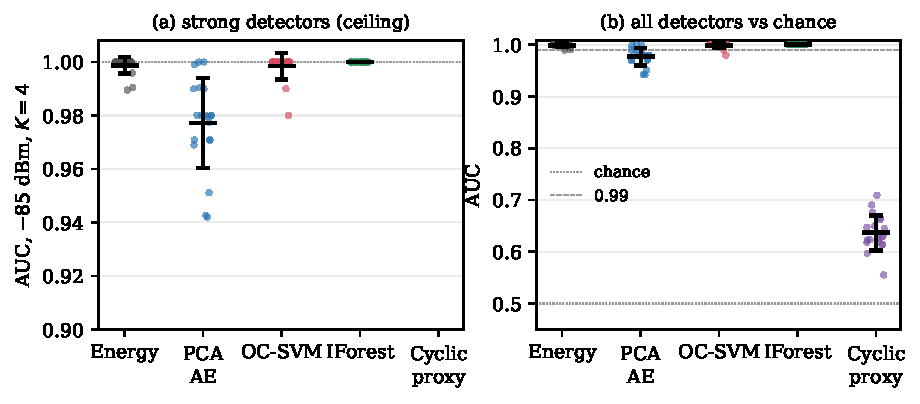
\includegraphics[width=\columnwidth]{figures/fig_auc_distribution.pdf}
\caption{Per-seed AUC for all twenty trials, with mean and one sample standard deviation. Panel (a) restricts the axis to show the strong detectors; the four are indistinguishable at the ceiling. Panel (b) shows all five against chance. Source: \Artifact{}.}
\label{fig:dist}
\end{figure}

The same ceiling appears in a single realisation at a larger sample size. Figure~\ref{fig:roc} plots the ROC curves of the 250/250/200 trial at $-85$ dBm, which the upstream code also persists---and whose own legend reads $1.000$, $1.000$, $1.000$, $1.000$ for the four strong detectors, not the $0.989$, $0.943$, and $0.999$ that the upstream text reports in the section citing this figure. We reproduce the curves here because they make the point visually: four of the five curves are mutually indistinguishable and pinned against the top of the unit square, so no ROC-based comparison between them is informative. We regenerate the point arrays with the committed code and commit them as \texttt{data/recovered\_roc.json}.

\begin{figure}[t]
\centering
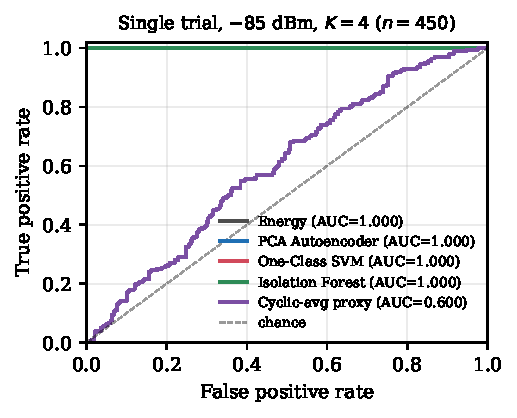
\includegraphics[width=\columnwidth]{figures/fig_roc_curves.pdf}
\caption{ROC curves at $-85$ dBm from a single 250/250/200 trial. The four strong detectors are mutually indistinguishable at the ceiling; only the cyclic proxy departs from it, and only slightly. These are the same numbers the upstream figure legend reports, and they contradict the values given in the upstream text that cites it. Source: \texttt{data/recovered\_roc.json}.}
\label{fig:roc}
\end{figure}

\section{Why the Benchmark Is Easy: a Spectrally Flat Nuisance Model}
\label{sec:mechanism}

The ceiling in Table~\ref{tab:mc} is not a property of anomaly detection; it is a property of the signal model. We established this by running targeted experiments against the committed generator.

The upstream manuscript describes the primary users as ``OFDM subcarriers at fixed centre frequencies of 2.4, 2.6, 5.2, and 5.8\,MHz.'' The generator implements each primary user as $\sqrt{p}\,e^{j(2\pi f_p t+\phi_n)}$ where $\phi_n$ is drawn \emph{independently for every sample}. A tone with a per-sample random phase is spectrally flat: it injects a broadband power excess and no spectral structure at all. Averaging the periodogram over forty realisations, the ratio of the maximum to the median bin power is $1.50$, consistent with a flat spectrum and inconsistent with four narrowband emitters, which would produce a contrast of one to two orders of magnitude at their centre frequencies. The simulated environment therefore contains no narrowband primary users, and the paper's spectral argument --- that the covert signal is detected through ``its localized power contribution to the spectrum'' --- describes a spectrum the code never produces.

The covert emission, by contrast, \emph{is} narrowband. Averaging the periodogram separately under $H_0$ and $H_1$ over sixty realisations each, the $H_1/H_0$ power ratio inside the covert band $(2.3,5.9)$\,MHz has median $3.41$ and maximum $8.21$, against a median of $1.05$ outside it. A localised excess exists. But because its centre frequency is redrawn uniformly for every observation, the excess moves, and no fixed subband feature, no fixed spectral statistic, and no fixed cyclic frequency can exploit it. The learnable, class-consistent evidence is the aggregate power excess, which is exactly the feature the energy baseline reads. This explains why the energy detector reaches AUC $0.9988$ at $-85$ dBm, and it explains the ceiling: the problem as generated is a total-power test, and a total-power test is easy when the two classes differ in total power.

\begin{table}[t]
\centering
\caption{Correlation between the upstream manuscript's quantitative claims and committed artifacts. ``Backed'' means a committed file supports the claim at the configuration cited.}
\label{tab:claims}
\small
\footnotesize
\setlength{\tabcolsep}{3.4pt}
\begin{tabular}{>{\raggedright\arraybackslash}p{0.44\columnwidth}>{\raggedright\arraybackslash}p{0.44\columnwidth}}
\toprule
Upstream claim & Audit outcome \\
\midrule
20-seed MC table, all 5 detectors & Backed. Reproduces to 4 decimals. \\
Isol. Forest AUC = 1.000 (body) & Backed. 1.0000 in 20/20 seeds. \\
Abstract: Isol. Forest AUC = 0.999 & False. Artifact gives 1.0000. \\
Body: Energy 0.989, AE 0.943, OC-SVM 0.999 & Wrong config. These are Monte Carlo trial~1, but the cited figure's own legend reads 1.000, 1.000, 1.000. \\
Cyclic proxy AUC = 0.600 & Other config. True only of the 250/250/200 trial; 20-seed mean is 0.6367. \\
Power range $-120$ to $-75$ dBm & False. Sweep ends at $-80$ dBm. \\
MC uses 250 train / 250 / 200 test & False. MC uses 100 train / 100 / 80 test. \\
``$-30$ dB window'' & False. 15 to 40 dB; two detectors never reach 0.99. \\
ML beats Energy by 5--10 dB, consistently & False. $+0$ and $+5$ dB; OC-SVM below baseline at 7 of 9 powers. \\
Monotonic gain with sensor count & False. Autoencoder drops 1.0000 to 0.9502 at $K=8$. \\
Energy needs $K=4$ to exceed 0.99 & False. Energy is 1.0000 at $K=1$. \\
Cyclic improves 0.55 to 0.65 with $K$ & False. 0.6500 at $K=1$ to 0.6990 at $K=8$; no 0.55 exists. \\
Fusion improves AUC by up to 0.15 & Unsupported. No artifact; not measured. \\
SNR $\approx P_c + 73$ dB & False by 46 dB. Correct: $P_c + 26.99$ dB. \\
Periodogram uses a Hann window & False. No window is applied. \\
Cyclic detector uses AC features & False. It uses columns 34--36; the cyclic code is never called. \\
Top features are psd\_max, band 2/3, psd\_p95 & False. The figure's own labels are different, and its top two entries are constant. \\
C kernel: ``under 1 s for 360 test obs'' & False. 2.0 s CPU, 260 observations, aborts at exit. \\
\bottomrule
\end{tabular}
\end{table}

\section{Distributed Fusion: a Null Result}
\label{sec:fusion}

The upstream package computes an AUC-versus-sensor-count series and discards it: the routine that draws the scalability figure never writes its values, and the saved artifact contains no sensor-indexed series. We regenerated it with the committed code at the committed call signature and commit it here as \texttt{data/recovered\_scalability.json}.

The result is a null. Four detectors score exactly $1.0000$ at \emph{every} $K$ from 1 to 8, including $K=1$. The autoencoder scores $1.0000$ at $K\leq4$ and \emph{drops} to $0.9502$ at $K=8$. The cyclic proxy is non-monotone, falling from $0.6500$ at $K=1$ to $0.6360$ at $K=2$ before rising to $0.7435$ at $K=4$ and falling again to $0.6990$ at $K=8$. There is no fusion gain to report, because a single sensor already separates the classes at this operating point. The upstream text's specific claims that gains are ``most dramatic'' between $K=1$ and $K=4$, that Energy Detection ``requires $K=4$ to exceed 0.99'', and that the cyclic proxy improves from $0.55$ at $K=1$ are each contradicted by the committed code; the value $0.55$ does not occur.

These points are also statistically weak in a way the upstream package does not acknowledge. The upstream routine reuses a \emph{single} environment object across all five methods and all four values of $K$, so the twenty runs are consecutive segments of one random stream. Each $(K,\text{method})$ cell is a different dataset; the $K=8$ dataset is not a superset of the $K=4$ dataset. Differences between adjacent $K$ values therefore confound fusion effect with data draw, with one realisation per cell and no dispersion. We report the series because it is real data, and we draw no conclusion from its shape beyond the absence of an effect at this operating point.

\begin{figure}[t]
\centering
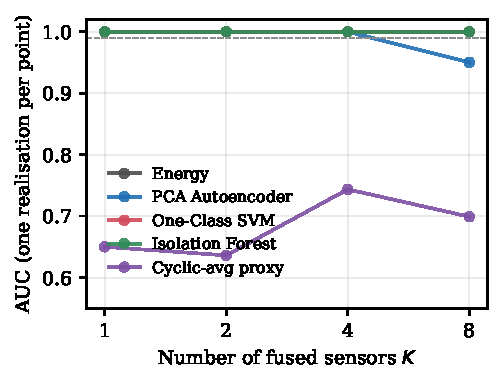
\includegraphics[width=\columnwidth]{figures/fig_auc_vs_sensors.pdf}
\caption{AUC against the number of fused sensors, regenerated with the committed code. One realisation per point, from an upstream routine that advances a single random stream across all twenty cells; points are not nested or paired. Four detectors are at AUC $1.0000$ for all $K$, so no fusion gain is visible. Source: \texttt{data/recovered\_scalability.json}.}
\label{fig:sensors}
\end{figure}

\section{Implementation Defects}
\label{sec:defects}

Four defects affect what the package can support. We report them because each bounds a claim.

\emph{The periodogram uses 2.5\,\% of the observation.} The manuscript states that a 512-point periodogram is computed with a Hann window over the snapshot. The code applies \emph{no} window and calls $\texttt{fft(signal, n=512)}$, which additionally truncates the 20480-sample observation to its first 512 samples. The spectral resolution actually used is $f_s/512=39.06$\,kHz, and 14 of the 41 features derive from those 512 samples alone, while the autocorrelation, envelope, and edge blocks use the full observation. The features are therefore not computed from a common observation.

\emph{Two of forty-one features are constant.} The autocorrelation at lag 0 is normalised by itself and is identically $1.0$; the accompanying max-over-lags statistic includes lag 0 and is also identically $1.0$. Both are constant, carry no information, and an ANOVA $F$-test returns $\texttt{NaN}$ for them. The upstream feature-importance routine sorts in descending order, which places $\texttt{NaN}$ first, so the two zero-information constants are plotted as the two most discriminative features. The upstream text then interprets the figure as ranking covert-discriminative features and names four specific features that do not appear on the figure's own axis. We exclude this figure from the present manuscript; there is no correct version of it to report.

\begin{table}[t]
\centering
\caption{Claim-to-artifact audit summary.}
\label{tab:summary}
\small
\begin{tabular}{>{\raggedright\arraybackslash}p{0.62\columnwidth}r}
\toprule
Quantitative claims in the upstream manuscript & 20 \\
\quad backed by a committed artifact & 3 \\
\quad contradicted by a committed artifact & 14 \\
\quad true only of a different configuration & 2 \\
\quad unsupported by any artifact & 1 \\
Figures with a committed generator and data & 3 of 5 \\
Detector ranking statistically resolvable & no \\
Fusion gain demonstrated & no \\
\bottomrule
\end{tabular}
\end{table}

\emph{The ``cyclostationary'' detector is not cyclostationary.} \label{sec:cyc} The manuscript derives a cyclic autocorrelation over 20 candidate cycle frequencies and then explains that the implementation substitutes ``the last six autocorrelation features (lags 0--20).'' Neither statement is accurate. The implementation's fallback path averages feature columns 34 to 36, which are a spectrogram texture statistic and two envelope-edge statistics, not autocorrelation values; the autocorrelation block occupies columns 25 to 30. The cyclic-autocorrelation method is present in the code but never invoked. The detector is a three-feature linear average, which is consistent with its near-chance performance ($0.6367$) and inconsistent with the manuscript's treatment of it as a deliberate efficiency approximation.

\emph{The C reference kernel is memory-unsafe and does not run.} The kernel's feature extractor writes 42 values into buffers declared with 41 elements, on every observation. AddressSanitizer reports a heap buffer overflow at the final write, and the overflow is observable directly: the value written for one training sample lands in the next sample's leading feature, corrupting the training matrix used to set the energy threshold. Every execution terminates with \texttt{SIGABRT} (exit status 134). The committed binary also prints an internally inconsistent result, reporting an AUC of $0.0000$ while simultaneously reporting $\mathit{P}_d=1.0000$ and $\mathit{P}_{fa}=0.0000$, at every power below saturation; a reimplementation of the same main routine with a correctly sized buffer returns $1.0000$, so the zero is a defect of the committed binary rather than a property of the method. The kernel additionally seeds from wall-clock time, so it is not reproducible; it hard-codes one feature to a placeholder; and its ``500\,kHz BPSK'' covert signal draws a fresh sign for every sample, making it a full-bandwidth random sequence. We exclude the kernel from all results in this paper.

\section{Limitations}
\label{sec:limit}

We state the limitations of this work and of the underlying evidence without hedging, because they determine what the evidence can support.

\emph{No prior-work comparison exists.} This is the most serious gap in the underlying evidence, and it is a gap in the audited package rather than in this audit. The package cites ten references and compares against none of them numerically. Every detector in Table~\ref{tab:mc} is an off-the-shelf one-class method applied to a self-generated feature set, and the only baseline is a total-power threshold defined inside the same codebase. A reader cannot tell whether the reported AUCs are competitive with published covert-detection or spectrum-anomaly results, because no such number is present. A detector paper without a prior-work comparison is a workshop contribution, not a conference contribution, and we do not present it as one. Establishing superiority would require implementing at least two published spectrum-anomaly or covert-detection methods against the same generator, plus cooperative-sensing baselines with AND/OR/$m$-out-of-$K$ voting, all evaluated on the same seeds. The package does contain hard, AND, OR, and $m$-out-of-$K$ fusion rules; none is evaluated in the artifacts.

\emph{This manuscript cites no prior work.} We have deliberately not supplied a reference list. We did not conduct a literature search, and the subject package's ten references were not independently verified. Stating the absence is more useful than filling it with plausible-looking citations, but the consequence is real: without positioning, this paper cannot establish novelty, and a reviewer should treat the novelty question as open.

\emph{The evidence is synthetic and single-scenario.} All results come from one generator with one noise floor, two primary users, one burst model, and one covert waveform family. There is no over-the-air data, no adversarial model of the detector, no non-stationary background, and no calibration error. The ceiling we report is a property of this generator.

\emph{The sweep and the sensor-count series are un-replicated.} Both carry one realisation per point, and the sensor-count series is additionally unpaired, with each cell drawn from a different segment of a shared random stream. We use them only to establish the absence of an effect at the reported operating point, never to characterise a trend.

\emph{The ceiling is not corrected for.} We did not select a harder operating point and re-run, because doing so would change the experiment rather than audit it. A fair positive study would fix the operating point in advance, for instance by requiring the energy baseline to sit near chance, and report dispersion there.

\section{Conclusion}
\label{sec:conclusion}

A twenty-seed anomaly-detection benchmark on simulated covert emissions is exactly reproducible, and that reproducibility is worth stating. Reproducibility, however, is not validity. At the operating point the package reports, the metric is saturated: the best detector is perfect in every seed, four of five detectors exceed $0.977$, and the paired per-seed differences between the leading candidates are zero in most trials, so the ranking the package reports is not recoverable from its own data. The reason is a modelling defect rather than a detector property: primary users generated with a per-sample random phase are spectrally flat, so the covert band is distinguished only by aggregate power and a total-power test suffices. In the only region where the problem is non-trivial, the machine-learning detectors do not beat the energy baseline consistently, and distributed fusion produces no measurable gain because one sensor already separates the classes.

The artifact-backed contributions of this paper are the recomputed twenty-seed table with dispersion and confidence intervals, the corrected account of the power sweep, the regeneration of a discarded sensor-count series, the spectral measurements that explain the ceiling, and the claim-to-artifact audit in Table~\ref{tab:claims}. The positive claim the audited package makes --- that anomaly detection is well suited to covert detection and that distributed fusion improves it --- is not supported by its artifacts, and we do not restate it. The minimum experiment set that would support it is: a prior-work baseline set on identical seeds; a spectrally valid primary-user model; replicated dispersion at a pre-registered operating point inside the transition region; a paired sensor-count design in which the $K=8$ dataset contains the $K=4$ dataset; a genuine cyclostationary implementation; and a feature-importance analysis computed against actual labels.

\section*{Manuscript History and Correction Notice}
\addcontentsline{toc}{section}{Manuscript History and Correction Notice}
The audited package (commit \texttt{3bf8a4d}) states in its abstract that the Isolation Forest achieves a system-level AUC of $0.999$ at $-85$ dBm, while its body states $1.000$. We verified the discrepancy and resolved it in favour of the artifact: \Artifact{} records an AUC of exactly $1.0000$ for Isolation Forest in all twenty of twenty seeds, so the abstract value is incorrect and the body value is correct. Where the upstream text reports Energy $0.989$, autoencoder $0.943$, and One-Class SVM $0.999$ in the same section, those are the values of Monte Carlo trial~1, whereas the figure that section cites was generated at a different sample size and its own legend reads $1.000$, $1.000$, and $1.000$. The upstream value $0.600$ for the cyclic proxy is not an error in the sense of being unreproducible: it is the single-trial result at 250/250/200, while the twenty-seed mean is $0.6367$ and the paired sweep point is $0.6266$. All values reported in this paper are the artifact values.

\end{document}
